\documentclass[11pt,twocolumn]{article}

\usepackage[utf8]{inputenc}
\usepackage[T1]{fontenc}
\usepackage{mathptmx}
\usepackage[a4paper,margin=2.3cm,columnsep=0.7cm]{geometry}
\usepackage{graphicx}
\usepackage{booktabs}
\usepackage{amsmath}
\usepackage{amssymb}
\usepackage{xcolor}
\usepackage{caption}
\usepackage{float}
\usepackage[hidelinks]{hyperref}
\usepackage{enumitem}
\usepackage{tabularx}
% Ragged-right auto-width column so wide tables wrap within \columnwidth
% instead of overflowing into the neighbouring column.
\newcolumntype{Y}{>{\raggedright\arraybackslash}X}

\graphicspath{{figures/}}
\captionsetup{font=small,labelfont=bf}
\setlength{\parindent}{1em}
\setlength{\parskip}{0.12em}
\renewcommand{\baselinestretch}{1.16}

\newcommand{\bt}[1]{\texttt{#1}}

% FAU logo pre-rendered into a box: \includegraphics cannot be called directly
% inside the \twocolumn[...] optional argument (fails with a \Gin@ii error), so
% we build the box here in the preamble and drop it into the title block below.
\newsavebox{\faulogobox}
\sbox{\faulogobox}{
\includegraphics[width=0.34\textwidth]{fau_logo.png}}

\title{\vspace{-1.2em}\textbf{Acoustic-Driven Generation of mFDA Clinical Speech\\
Reports with Flan-T5: Reproduction, Optimisation, and a\\
Study of Evaluation-Metric Comparability}\\[0.3em]
\large Final Project Report}
\author{}
\date{}

\begin{document}
\twocolumn[
\begin{@twocolumnfalse}
\begin{center}
\usebox{\faulogobox}
\end{center}
\vspace{0.2em}
\maketitle
\vspace{-2.5em}
\begin{center}
\normalsize Author: Dawood Aijaz \quad$\cdot$\quad Matriculation Number: 23282229 \quad$\cdot$\quad Date: July 13, 2026
\end{center}
\vspace{0.6em}
\begin{abstract}
\noindent
Clinical speech assessment for Parkinson's disease (PD) relies on perceptual scales such as
the modified Frenchay Dysarthria Assessment (mFDA), which are subjective, expert-intensive,
and rarely produce standardised written reports. Building on the reference study of
Arias-Vergara et al., this project fine-tunes sequence-to-sequence language models to generate
mFDA-style clinical reports directly from seven numeric acoustic biomarkers (breathing, lips,
palate, larynx, monotonicity, tongue, and intelligibility). Training uses a large synthetic
corpus of simulated biomarker--report pairs; the held-out test set consists of real PD and
healthy-control (HC) clinical reports. Through a reproducible extraction--preparation--training
--evaluation pipeline and more than twenty controlled experiments, we identify a best
configuration, \emph{B17}: a 248M-parameter Flan-T5-base model adapted with rank-32 LoRA.
Our central finding is methodological: the apparent gap between our Flan-T5 model and the
reference paper's headline scores is \emph{mostly a measurement artifact}, not a model
deficiency. The reference evaluation reports character-level BLEU, whereas standard practice
uses word-level BLEU; on the same generated text the two differ by roughly a factor of two.
After reproducing the original evaluation exactly---character-level BLEU-2, stemmed ROUGE, and
an English BERTScore backbone---B17 attains an average score of \textbf{0.649} (character-BLEU
0.759, BERTScore 0.911), placing a 248M model beside the reference paper's best
seven-billion-parameter systems. We further map the Flan-T5-base performance plateau across
learning rate, epochs, weight decay, label smoothing, model size, LoRA rank, oversampling,
structured targets, and encoder-input format, and we correct a BERTScore language
misconfiguration that had systematically undervalued semantic scores. We conclude that B17 is
final for the Flan-T5 track and that surpassing the reference headline requires a
decoder-only 7B model rather than further small-model tuning.
\end{abstract}
\vspace{1.0em}
\end{@twocolumnfalse}
]

\section{Introduction}

\subsection{Motivation}
Speech is a rich, non-invasive biosignal that reflects many aspects of neurological health.
In Parkinson's disease (PD), progressive motor impairment frequently produces
\emph{dysarthria}---a motor speech disorder caused by weakness, slowness, or poor coordination
of the muscles used for speaking. Despite its diagnostic relevance, speech is seldom formally
assessed in routine PD evaluation, in part because standardised written reporting protocols are
uncommon and because expert perceptual rating is time-consuming and inconsistent between raters.

The modified Frenchay Dysarthria Assessment (mFDA) is one of the few instruments that quantify
speech impairment in a structured way. It scores seven perceptual categories---breathing, lips,
palate, larynx, monotonicity, tongue, and overall intelligibility---each on an ordinal scale
that an expert phoniatrician maps from ``normal'' to ``severe.'' While clinically meaningful,
the assessment is subjective and demanding: it requires trained listeners and does not directly
yield a narrative report a clinician can read, share, or archive.

Two complementary difficulties motivate an automated approach. Purely acoustic analysis produces
numeric biomarkers that are objective but hard to interpret without signal-processing expertise;
purely perceptual assessment produces interpretable judgements but is labour-intensive. Large
language models (LLMs) offer a bridge: given objective acoustic biomarkers as input, a fine-tuned
model can emit a structured, human-readable clinical report, combining the objectivity of
acoustics with the interpretability of narrative text. Crucially, the acoustic biomarkers act as
an explicit, controllable input the clinician can inspect---unlike an end-to-end black box that
maps audio directly to text---so the generation remains auditable.

\subsection{Task and reference study}
This project reproduces and extends the study \emph{``Acoustic-Driven Generation of Pathological
Speech Reports Using Large Language Models''} (Arias-Vergara et al., 2025). The reference work
frames report generation as a text-to-text problem: seven acoustic biomarkers, correlated with
the seven mFDA categories, are formatted into an input prompt, and a fine-tuned LLM generates an
mFDA-style report as output. Because only 50 PD and 50 HC subjects are available---far too few to
train a generative model---the authors introduce a data-augmentation strategy that
\emph{simulates} biomarker--report pairs from the statistical distribution of the real features,
yielding a large synthetic training corpus. Real subject reports are reserved exclusively for
testing, avoiding overfitting to the small clinical set.

The reference study fine-tunes a range of models (T5, Flan-T5, GPT-2, LLaMA-7B, Mistral-7B, and
a DeepSeek 7B variant) and reports generation quality with ROUGE, BLEU, and BERTScore. Its
headline result is that the best (seven-billion-parameter) models reach BLEU scores of 0.789 for
PD and 0.836 for HC, with smaller encoder--decoder models such as T5 and Flan-T5 scoring lower.
Our work focuses on the encoder--decoder family---specifically Flan-T5---because it is compact,
reproducible on a single GPU, directly controllable through prompt design, and a realistic target
for deployment in resource-constrained clinical settings.

\subsection{Contributions}
This report makes four contributions:
\begin{enumerate}[leftmargin=1.3em,itemsep=0.15em,topsep=0.2em]
  \item A fully reproducible, three-stage pipeline (ETL $\rightarrow$ prepare $\rightarrow$
        train/eval) with a single parsing core, deterministic hashing, and a cross-split leakage
        guard.
  \item A best Flan-T5 configuration, \emph{B17} (Flan-T5-base $+$ rank-32 LoRA), together with
        an exhaustive map of \emph{closed} training levers so future work does not re-explore
        saturated axes.
  \item A demonstration that the apparent gap to the reference headline is \emph{mostly a
        measurement artifact}: reproducing the paper's exact character-level BLEU and correcting
        a BERTScore language misconfiguration raises the same model's score from ``far behind''
        to competitive with 7B systems.
  \item An open, standardised evaluation harness with two explicit rulers---an honest,
        widely-comparable one for model selection and an author-parity one for fair comparison
        against the reference paper.
\end{enumerate}

\subsection{Objectives and scope}
\subsubsection{Objectives}
\begin{itemize}[leftmargin=1.1em,itemsep=0.12em,topsep=0.2em]
  \item Build a reproducible pipeline from raw biomarker--report CSVs to tokenised training
        batches, fine-tuned checkpoints, and metric reports.
  \item Reproduce the reference Flan-T5 result and search for a configuration that matches or
        improves upon it under a fair, standardised evaluation.
  \item Diagnose \emph{why} our Flan-T5 scores appeared far below the reference headline, and
        establish whether the gap reflects the model or the measurement.
  \item Map which training levers help, which regress, and where the Flan-T5-base family
        plateaus.
\end{itemize}

\subsubsection{Scope}
\begin{itemize}[leftmargin=1.1em,itemsep=0.12em,topsep=0.2em]
  \item We use the biomarker--report CSV splits supplied with the project; audio feature
        extraction is upstream and out of scope, though we summarise it for completeness.
  \item The work targets \emph{supervised text generation} with encoder--decoder transformers,
        not decoder-only 7B models (discussed only as a comparison ceiling).
  \item Experiments are designed for reproducible single-node, mixed-precision training on
        NVIDIA A100 GPUs.
  \item Model selection is reported primarily with a standardised decode metric, with a second
        evaluation reproducing the reference paper's exact metric definitions for comparability.
\end{itemize}

\section{Background and Related Work}

\subsection{T5 and Flan-T5 encoder--decoder models}
The Text-to-Text Transfer Transformer (T5) casts every NLP problem as text-to-text, using a
unified encoder--decoder transformer trained with a span-corruption objective. Flan-T5 augments
T5 with large-scale instruction fine-tuning, improving zero- and few-shot behaviour and making
the model more responsive to natural-language task prefixes. For biomarker-to-report generation,
Flan-T5 is attractive: the encoder ingests a short, structured prompt describing the seven
biomarkers, and the decoder emits the report autoregressively under teacher forcing. Within a
size tier, T5 and Flan-T5 share a tokenizer vocabulary, which simplifies experimentation; our
own ablation confirms that the instruction-tuned Flan variant substantially outperforms plain
T5 at base scale (Section~\ref{sec:results}).

Fine-tuning optimises the token-level cross-entropy of the reference report under teacher
forcing. For a target sequence $y_{1:T}$ conditioned on the encoder input $x$,
\begin{equation}
\mathcal{L}(\theta) = -\frac{1}{T}\sum_{t=1}^{T} \log p_\theta\!\left(y_t \mid y_{<t}, x\right),
\end{equation}
where padding positions are masked (label $-100$) so they do not contribute to the loss. Weight
decay is applied to the parameters as regularisation; it is not part of the sequence objective.

\subsection{Decoding strategies}
At inference, the decoder must turn the learned distribution into text. \emph{Beam search}
maintains the $k$ highest-probability partial sequences and is deterministic; it favours
high-likelihood, often generic text. \emph{Sampling} (with temperature and top-$k$/top-$p$
truncation) injects controlled randomness, producing more varied text at the cost of
reproducibility. A subtle but important point for this project is that the reference paper and our
standardised evaluation use \emph{different} decoding: the reference samples with a minimum-length
constraint, while our selection metric uses deterministic beam search. Decoding choices interact
with metrics---for example, a minimum-length constraint inflates recall-oriented scores---so both
must be held fixed when comparing systems.

\subsection{Parameter-efficient fine-tuning (LoRA)}
Full fine-tuning updates all weights, which is costly and prone to overfitting on small or
repetitive corpora. Low-Rank Adaptation (LoRA) freezes the pretrained weight $W_0$ and learns a
low-rank update,
\begin{equation}
W = W_0 + \frac{\alpha}{r}\, B A,\qquad B\in\mathbb{R}^{d\times r},\ A\in\mathbb{R}^{r\times k},
\end{equation}
with rank $r \ll \min(d,k)$, so only $BA$ is trained. Adapters can be merged into $W_0$ after
training, so downstream inference and evaluation code need not change. In this project LoRA
provides a small but consistent improvement over full fine-tuning at base scale and is the
mechanism behind our best model.

\subsection{Evaluation metrics for generated text}
\label{sec:metrics-bg}
Three families of metric are standard for report generation and are used by the reference study.
\emph{ROUGE} measures $n$-gram overlap between hypothesis and reference; we report ROUGE-1,
ROUGE-2, and ROUGE-L F-measures. \emph{BLEU} is a precision-oriented $n$-gram metric with a
brevity penalty (BP):
\begin{equation}
\mathrm{BLEU} = \mathrm{BP}\cdot\exp\!\Big(\textstyle\sum_{n=1}^{N} w_n \log p_n\Big),
\end{equation}
where $p_n$ is the modified $n$-gram precision. \emph{BERTScore} embeds hypothesis and reference
tokens with a pretrained language model and aligns them by cosine similarity, giving partial
credit for paraphrase where surface overlap is low.

A recurring, easily overlooked pitfall---central to this report---is that ``BLEU'' is not a
single number. Two implementation choices dominate. First, the \emph{unit}: word-level BLEU-4
(the SacreBLEU standard, $N{=}4$) versus character-level BLEU-2 ($N{=}2$ over characters) can
differ by roughly a factor of two on the same text, because character $n$-grams overlap far more
than word $n$-grams for texts that share an alphabet and boilerplate. Second, the \emph{BERTScore
backbone language}: scoring English text with a multilingual/Spanish backbone yields
systematically lower values than with an English backbone. Both issues turn out to explain most
of the apparent gap between our model and the reference headline, and both are invisible unless
the exact metric implementation is reproduced rather than merely named.

\subsection{Automatic medical report generation}
Automatic medical report generation (aMRG) is an established area, typically combining a
domain-specific encoder with a text decoder; most prior work targets imaging modalities. The
reference study is, to our knowledge, the first to extend aMRG to \emph{pathological speech},
treating acoustic biomarkers---rather than pixels---as the primary evidence for a generated
clinical narrative. Our contribution is not a new architecture but a rigorous reproduction,
optimisation, and, most importantly, a clarification of how these systems should be measured and
compared.

\section{Data and Problem Formulation}

\subsection{Dataset and mFDA annotation structure}
The clinical data derive from the PC-GITA corpus: 50 PD patients (25 male, 25 female) and 50 HC
speakers (25 male, 25 female), all Colombian-Spanish native speakers (mean age
$61.9\pm9.6$ for PD and $60.9\pm9.5$ for HC), recorded across four speech tasks (sustained
phonation of /a/, /pa-ta-ka/ diadochokinetic repetition, text reading, and spontaneous
conversation) and resampled to 16\,kHz. Expert phoniatricians rate the seven mFDA categories from
0 (normal) to 4 (severe); the median of three raters is used and mapped to a categorical
severity: $0$--$1\rightarrow$ Normal, $2\rightarrow$ Mild, $3\rightarrow$ Moderate, and
$4\rightarrow$ Severe. Notably, although the \emph{speech} is Spanish, the mFDA \emph{reports}
themselves are written in \emph{English}---a fact that later proves decisive for BERTScore
configuration.

\subsection{Acoustic biomarkers}
Although feature extraction is upstream of our pipeline, understanding the input is essential.
The reference work computes 248 task-specific acoustic biomarkers (no denoising; amplitudes
scaled to $[-1,1]$ and centred) and selects the most relevant features per mFDA category using a
statistical approach. The features fall into three groups, each mapped to particular mFDA
categories and speech tasks (Table~\ref{tab:biomarkers}): \emph{phonation} features (pitch $F_0$
standard deviation, sound-pressure level, jitter, shimmer) reflect voice-source stability;
\emph{prosody} features (pitch/SPL variation, pause statistics, voiced/voiceless ratios) capture
melody, rhythm, and timing; and \emph{phonemic} features (pronunciation precision, phoneme-class
duration and rate, the pairwise variability index, and articulation-group statistics) describe
articulatory precision. In our pipeline these are already reduced to the seven per-category
values that form the model input.

\begin{table}[t]
\centering
\caption{Acoustic feature groups and their mapping to mFDA categories.}
\label{tab:biomarkers}
\small
\begin{tabular}{@{}p{1.35cm}p{2.1cm}p{2.6cm}@{}}
\toprule
Group & Focus & mFDA categories \\
\midrule
Phonation & Voice-source stability \& loudness & Larynx \\
Prosody & Melody, rhythm, timing & Monotonicity, Breathing \\
Phonemic & Articulatory precision & Lips, Tongue, Palate, Intelligibility \\
\bottomrule
\end{tabular}
\end{table}

\subsection{Simulation strategy and splits}
Because only 100 subjects exist, the reference augmentation strategy simulates biomarkers from
the real feature distributions and pairs them with templated mFDA reports, producing a synthetic
corpus of roughly 110{,}000 pairs. The synthetic prompts follow a balanced severity design
(Figure~\ref{fig:severity}): 25\% carry random ratings across all categories, 25\% Normal--Mild,
25\% Mild--Moderate, and 25\% Moderate--Severe, ensuring that the model sees the full severity
range rather than a narrow, easy distribution. The project provides synthetic train sizes of 1k,
10k, and 100k pairs, a 10k synthetic validation split, and a held-out test split of
\textbf{96 real reports} (48 PD, 48 HC). Real data is used only for testing.

\begin{figure}[t]
\centering
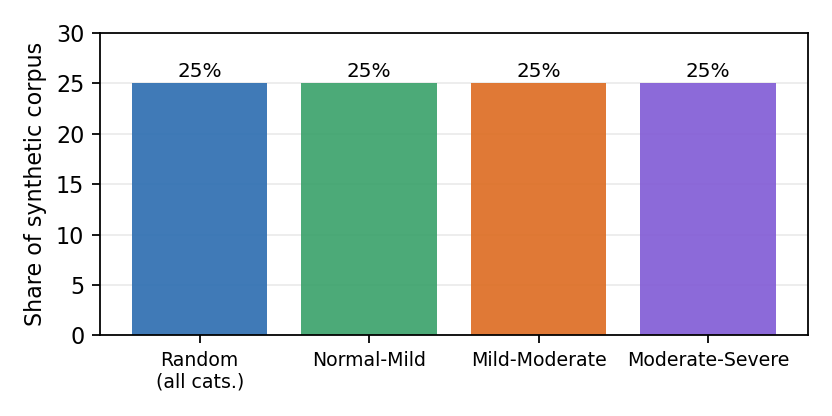
\includegraphics[width=0.92\columnwidth]{fig_severity.png}
\caption{Balanced severity design of the synthetic corpus: equal shares of random, Normal--Mild,
Mild--Moderate, and Moderate--Severe reports, so the model observes the full severity range.}
\label{fig:severity}
\end{figure}

\subsection{ETL and exploratory data analysis}
A dedicated extraction--transformation--loading (ETL) stage is the single source of truth for
schema normalisation. It loads the raw CSV splits, normalises the differing simulated and real
schemas into one canonical schema, and---critically---parses the seven biomarkers out of the raw
\bt{Instructions} string into numeric columns in a fixed order (breathing, lips, palate, larynx,
monotonicity, tongue, intelligibility). Each row is assigned a deterministic
\bt{example\_hash}$=$SHA-256 of the concatenated input and target, enabling reproducible
deduplication and a cross-split leakage guard so that no test report leaks into training. The
canonical schema retains provenance (\bt{sample\_id}, \bt{source\_file}, \bt{source\_row}), group
labels (PD/HC/None), the parsed floats, and both the normalised \bt{input\_text} and
\bt{target\_text}.

\begin{table}[t]
\centering
\caption{Report-structure audit across splits: all seven mFDA slots are present in every report,
but synthetic targets are far more repetitive than real ones.}
\label{tab:audit}
\small
\begin{tabular}{lcccc}
\toprule
Split & $n$ & Coverage & Median len & Dup.\ rate \\
\midrule
Train (syn.) & 99{,}893 & 1.00 & 494 & 0.949 \\
Val (syn.)   & 10{,}000 & 1.00 & 494 & 0.845 \\
Test (real)  & 96       & 1.00 & 438 & 0.500 \\
\bottomrule
\end{tabular}
\end{table}

An audit of the prepared splits (Table~\ref{tab:audit}) confirms that every report---synthetic
and real---contains all seven \bt{Category (Severity)} slots (coverage 1.0). Median target length
is 494 characters for synthetic reports and 438 for real reports (PD reports are longer, median
478, than HC, median 404). The synthetic training targets have a high duplicate rate (0.95),
reflecting the templated, memorisable phrasing of simulated reports; the real test reports are
far more varied (duplicate rate 0.5). This distribution mismatch---clean, repetitive training
text versus varied clinical prose---partly explains why the model reproduces coarse structure
well but struggles with the exact wording of held-out real reports, and it bounds the achievable
overlap-based scores independently of model capacity.

\subsection{Input/output formulation and prompt design}
The model does not consume a continuous feature vector; it consumes \emph{text}. The ETL parses
the seven numbers and formats them into a compact, fixed-order \bt{input\_text} (for example,
\bt{Breathing: 78 Lips: 1.75 Palate: 0.94 \dots}). A task prefix is prepended to form the encoder
\bt{source\_text}. The decoder target is the mFDA report string. Padding positions in the labels
are masked to $-100$.

We implemented five prompt styles: a default mFDA instruction; \bt{flan-paper} (the reference
prefix ``Generate a report for:''); a variant with explicit category hints; a variant with
deterministic \bt{Category=value} numeric labels; and a variant that supplies a seven-slot output
template. As shown in Section~\ref{sec:results}, the concise \bt{flan-paper} prompt over the
compact seven-score input is the strongest; more elaborate prompts and the raw, unparsed
\bt{Instructions} string both regress. Intuitively, the compact numeric prompt gives the encoder
a clean, low-noise view of exactly the seven quantities that matter, whereas the raw instruction
string dilutes that signal with free-text scaffolding.

\section{Methods}

\subsection{Overall pipeline}
The system is organised as three sequential, independently reusable stages that share the single
ETL parsing core, so no component re-parses raw strings (Figure~\ref{fig:pipeline}):
\emph{ETL} produces canonical Parquet/JSONL with parsed features and hashes; \emph{prepare} wraps
the canonical splits in a T5 prompt and tokenises them into a Hugging Face \bt{DatasetDict}
(\bt{input\_ids}, \bt{attention\_mask}, and masked \bt{labels}), saved to disk for fast reuse;
\emph{train} runs a \bt{Seq2SeqTrainer}; and \emph{eval} decodes the real test split and computes
generation metrics. Because \bt{prepare} calls the same ETL loader, it can read raw CSVs directly
without a separate ETL pass, which keeps the two entry points consistent by construction.

\begin{figure}[t]
\centering
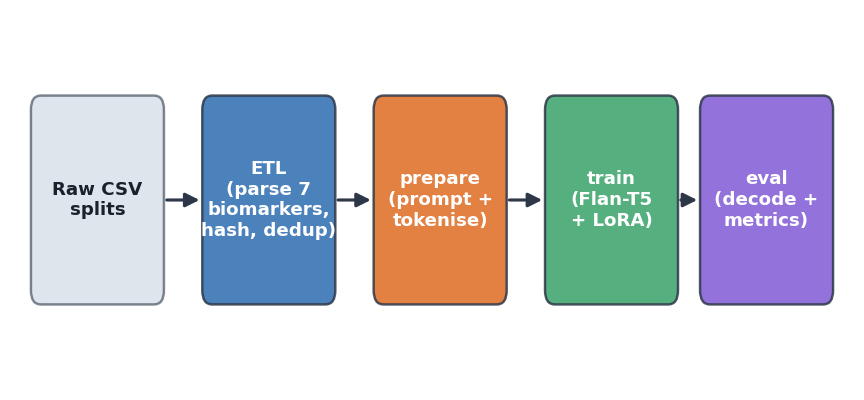
\includegraphics[width=\columnwidth]{fig_pipeline.png}
\caption{The three-stage pipeline. A single ETL parsing core feeds both the batch ETL and the
per-run \bt{prepare} stage, guaranteeing identical feature parsing everywhere.}
\label{fig:pipeline}
\end{figure}

\subsection{Software architecture}
The implementation is organised into small, single-responsibility modules so that every stage is
independently testable and reusable. The ETL core (\bt{etl/etl\_lib.py}) owns all schema
normalisation, biomarker parsing, hashing, and deduplication; \bt{etl/run\_etl.py} batches it
across train sizes and adds the cross-split leakage guard. In the training package,
\bt{main/prompts.py} defines the fixed seven-category order and all prompt styles;
\bt{main/tokenization.py} builds and tokenises the \bt{DatasetDict}; \bt{main/train.py} wraps
\bt{Seq2SeqTrainer} and implements LoRA, encoder freezing, and oversampling;
\bt{main/eval\_decode.py} and \bt{main/eval\_author\_parity.py} implement the two evaluation
rulers; and the \bt{structured\_*} and \bt{report\_severity} modules implement the seven-slot
structured path. Because the same parsing order is imported everywhere, the seven categories are
guaranteed to be consistent across parsing, prompting, and structured generation---a small but
important guard against silent misalignment.

\subsection{Model and fine-tuning}
The backbone is \bt{google/flan-t5-base} (248M parameters), chosen after confirming that the
instruction-tuned Flan variant clearly beats plain T5-base at the same recipe. Fine-tuning uses
token-level cross-entropy (teacher forcing) with AdamW and weight decay. Two adaptation modes are
supported: full fine-tuning and LoRA. Our best model, \emph{B17}, first full-fine-tunes for five
epochs (the ``B11'' checkpoint) and then applies rank-32 LoRA for three further epochs; the LoRA
adapters are merged into the exported \bt{final\_model} so that evaluation is identical to a plain
checkpoint. A \bt{--freeze-encoder} decoder-only mode and severity-based oversampling are also
implemented for ablations.

\subsection{Tokenisation and training loop}
The \bt{prepare} stage tokenises \bt{source\_text} and \bt{target\_text} with the model's
tokenizer, truncating and padding to \bt{max\_source\_length}$=256$ and
\bt{max\_target\_length}$=512$, then rewrites padding label ids to $-100$. Training uses
\bt{Seq2SeqTrainer} with step-based evaluation on the synthetic validation split,
\bt{load\_best\_model\_at\_end}, warmup ratio 0.1, and a rolling checkpoint limit. A key
methodological lesson, established repeatedly in our logs, is that \emph{teacher-forcing
validation loss is not a reliable selection criterion}: loss and generation quality diverged
several times (for example, a checkpoint with near-zero synthetic validation loss did not
maximise decode quality). We therefore select checkpoints by decode AVG from \bt{eval\_decode},
not by validation loss (Figure~\ref{fig:curves}).

\subsection{Prompt engineering and structured targets}
Beyond prompt prefixes, we explored a ``structured'' path that forces free text into a mandatory
seven-slot \bt{Category (Severity): description} skeleton, and a compact label-only target
(\bt{Category: Severity}) scored separately for label accuracy. These were motivated by the
observation that generated reports often omit explicit slot structure. As reported below, neither
structured post-processing, structure-aware re-ranking, nor training directly on label-only
targets improved decode quality over B17; training on label-only targets in fact reduced it
sharply.

\subsection{Evaluation methodology}
\label{sec:evalmethod}
We deliberately maintain \emph{two} evaluation scripts, because the choice of metric is itself a
result of this project.

\textbf{Honest evaluation} (\bt{eval\_decode}) uses standardised, widely comparable settings:
word-level SacreBLEU-4 (13a tokenizer) reported on $[0,1]$, ROUGE via the \bt{evaluate} library
(bootstrap-aggregated F1), BERTScore mean F1, and deterministic beam search (beam 3, 512 tokens,
no-repeat-$n$-gram 2). This is the metric used for \emph{model selection}, and the AVG column is
the simple mean of R-1, R-2, R-L, BLEU, and BERT, matching the reference paper's Table 4 summary.

\textbf{Author-parity evaluation} (\bt{eval\_author\_parity}) reproduces the reference paper's
exact evaluation code: character-level BLEU-2 (the reference passes raw strings to
\bt{nltk.sentence\_bleu} with weights $(0.5,0.5)$, which tokenises into characters), stemmed
per-example ROUGE F1, an English BERTScore backbone, and the reference sampling decode
(\bt{do\_sample}, temperature 0.7, top-$k$ 50, \bt{min\_length}$=100$, beam 3). This script exists
solely to compare fairly against the reference numbers; it is never used to select models.
Crucially, both scripts feed each model the input format it was trained on, so the comparison
isolates the metric rather than confounding it with input changes. The parity script also degrades
gracefully if the BERTScore backbone is unavailable offline, emitting BLEU and ROUGE with an
explicit status flag rather than failing.

\begin{table}[t]
\centering
\caption{Reference (author-parity) generation settings versus our honest decode settings.}
\label{tab:decode}
\small
\begin{tabular}{lll}
\toprule
Setting & Honest & Author-parity \\
\midrule
BLEU & word BLEU-4 & char BLEU-2 \\
ROUGE stemmer & off & on \\
BERTScore lang & en & en \\
Decoding & beam 3 & sample, beam 3 \\
Min length & --- & 100 \\
Temperature / top-$k$ & --- & 0.7 / 50 \\
\bottomrule
\end{tabular}
\end{table}

\subsection{Training procedure and hyperparameters}
Table~\ref{tab:config} lists the principal configuration of the best model. The best base recipe
uses learning rate $5\mathrm{e}{-}4$, weight decay 0.01, warmup 0.1, and five epochs at 100k; the
LoRA stage adds three epochs at rank 32. Runs execute on NVIDIA A100 (40\,GB) nodes of an HPC
cluster; on older V100 hardware we avoid FP16 because of historical numerical instability, using
FP32 instead.

\begin{table}[t]
\centering
\caption{Principal training configuration for the best model (B17).}
\label{tab:config}
\small
\begin{tabularx}{\columnwidth}{@{}lY@{}}
\toprule
Setting & Value \\
\midrule
Base model & \bt{google/flan-t5-base} (248M) \\
Adaptation & 5-epoch full FT $+$ LoRA rank 32, 3 ep \\
Prompt style & \bt{flan-paper} (``Generate a report for:'') \\
Encoder input & compact seven-score string \\
Learning rate & $5\mathrm{e}{-}4$ \\
Weight decay & 0.01 \\
Warmup ratio & 0.1 \\
Batch size (train/eval) & 4 / 4 per device \\
Max source / target length & 256 / 512 tokens \\
Optimiser & AdamW, cross-entropy loss \\
Train / val / test & 100k / 10k / 96 \\
Hardware & NVIDIA A100 40\,GB (TinyGPU) \\
Selection criterion & decode AVG (\bt{eval\_decode}) \\
\bottomrule
\end{tabularx}
\end{table}

\section{Experiments and Results}
\label{sec:results}

\subsection{Experimental setup}
All runs are labelled with identifiers (\emph{B}$n$ for Flan-T5-base; \emph{S}, \emph{L},
\emph{N} prefixes for small, large, and non-Flan) and logged consistently across recipe, results,
and roadmap documents. Every finished run produces a \bt{test\_decode\_metrics.json} with
per-metric and PD/HC breakdowns. Metrics are computed on the 96 real reports; the paper's own
Table 4 uses 100 real reports, so absolute numbers should be compared with that small difference
in mind. We organise the search into phases: learning rate and epochs (Phase 1), prompt design
(Phase 2), decoding (Phase 3), parameter-efficient adaptation (Phase 4), structured generation
(Phase 5), and encoder-input format (Phase 6).

\subsection{Quantitative results}
Tables~\ref{tab:honest} and~\ref{tab:parity} present the best model (B17) under the two rulers.
Under the \emph{honest} ruler (Table~\ref{tab:honest}), B17 reaches an overall AVG of 0.559, with
word-level BLEU of 0.362 and BERTScore of 0.911. Under the \emph{author-parity} ruler
(Table~\ref{tab:parity})---the reference paper's exact metrics---the same model reaches AVG 0.649,
with character-level BLEU of 0.759 and BERTScore of 0.911.

\begin{table}[t]
\centering
\caption{B17 under the \emph{honest} ruler (\bt{eval\_decode}): word-level SacreBLEU-4, ROUGE,
BERTScore (\bt{lang=en}), deterministic beam search.}
\label{tab:honest}
\small
\begin{tabular}{lcccccc}
\toprule
Group & R-1 & R-2 & R-L & BLEU & BERT & AVG \\
\midrule
Overall & 0.605 & 0.389 & 0.530 & 0.362 & 0.911 & \textbf{0.559} \\
PD      & 0.582 & 0.336 & 0.491 & 0.342 & 0.909 & 0.532 \\
HC      & 0.625 & 0.441 & 0.569 & 0.383 & 0.914 & 0.586 \\
\bottomrule
\end{tabular}
\end{table}

\begin{table}[t]
\centering
\caption{B17 under the \emph{author-parity} ruler (\bt{eval\_author\_parity}): character-level
BLEU-2, stemmed ROUGE, BERTScore (\bt{lang=en}), reference sampling decode. Compare
these---not Table~\ref{tab:honest}---to the reference paper's numbers.}
\label{tab:parity}
\small
\begin{tabular}{lcccccc}
\toprule
Group & R-1 & R-2 & R-L & BLEU & BERT & AVG \\
\midrule
Overall & 0.632 & 0.394 & 0.548 & \textbf{0.759} & 0.911 & \textbf{0.649} \\
PD      & 0.611 & 0.344 & 0.508 & 0.744 & 0.909 & 0.623 \\
HC      & 0.652 & 0.444 & 0.588 & 0.775 & 0.912 & 0.674 \\
\bottomrule
\end{tabular}
\end{table}

For reference, the paper reports BLEU 0.789 (PD) and 0.836 (HC) for its best
seven-billion-parameter systems, and an overall average of roughly 0.68 for LLaMA-7B. B17's
parity numbers (character-BLEU 0.744/0.775; AVG 0.649) therefore sit within a few points of
models roughly \emph{28$\times$ larger}, from a 248M encoder--decoder.

\begin{figure}[t]
\centering
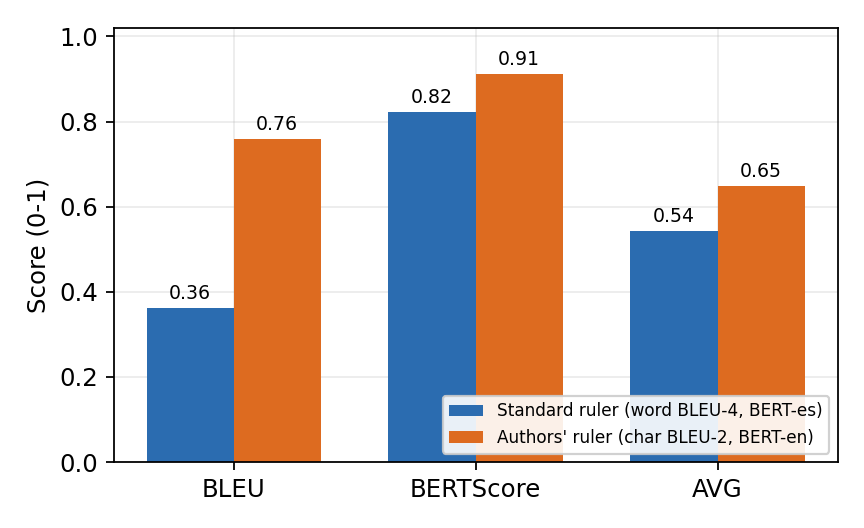
\includegraphics[width=\columnwidth]{fig_metric_artifact.png}
\caption{The same B17 outputs scored under two rulers. Switching from word-level to
character-level BLEU nearly doubles the BLEU score; correcting the BERTScore backbone from a
multilingual (\bt{es}) to an English (\bt{en}) model raises BERTScore. Neither changes a single
generated word.}
\label{fig:artifact}
\end{figure}

\subsection{The apparent paper gap is mostly the metric}
Figure~\ref{fig:artifact} isolates the effect. The identical B17 generations read as BLEU 0.362
(word-level) or BLEU 0.759 (character-level)---a difference of roughly a factor of two---driven
entirely by the metric definition. As an illustration on our own data, scoring two \emph{different}
real reports against each other already yields character-BLEU-2 near 0.84, because English
clinical reports share an alphabet and heavy boilerplate; the metric therefore mostly measures
language overlap, not report-specific correctness. A decisive cross-check is ROUGE-2, which is
nearly identical under both rulers (0.389 honest vs.\ 0.394 parity) because ROUGE is word-based in
both cases; the divergence lives \emph{only} in BLEU, exactly as the character-versus-word
explanation predicts. This confirms that the ``gap'' is a measurement choice, not weaker
generation.

To make the effect fully concrete, Table~\ref{tab:bleu-demo} scores two \emph{arbitrary,
different} real reports against each other---not a model output at all---under three BLEU
variants. The character-level BLEU-2 used by the reference evaluation reads 0.84, while standard
word-level BLEU-4 reads 0.43 for the very same pair. In other words, the reference metric assigns
a high score simply for two English clinical reports sharing an alphabet and template phrasing;
much of what it rewards is language and boilerplate overlap rather than report-specific
correctness. This is why the metric choice, not the model, dominates the comparison with the
reference paper.

\begin{table}[t]
\centering
\caption{Three BLEU variants on the \emph{same} pair of two different real reports (a lower bound
that involves no model). Character-level BLEU-2---the reference metric---roughly doubles the
standard word-level BLEU-4.}
\label{tab:bleu-demo}
\small
\begin{tabular}{lc}
\toprule
BLEU variant & Score \\
\midrule
Character-level BLEU-2 (reference metric) & 0.84 \\
Word-level BLEU-2 & 0.52 \\
Word-level BLEU-4 (standard) & 0.43 \\
\bottomrule
\end{tabular}
\end{table}

\subsection{The BERTScore language correction}
A second measurement issue was a misconfigured BERTScore backbone. The evaluation had defaulted
to a Spanish/multilingual model (\bt{lang=es}) because the source speech is Spanish---but the
reports are English. Re-scoring B17 with the correct English backbone (\bt{lang=en},
RoBERTa-large) raised BERTScore from 0.823 to 0.911 and the honest AVG from 0.542 to 0.559, with
ROUGE and BLEU unchanged to the reported digits---again the signature of a pure metric correction.
We fixed the default across all evaluation entry points and annotated the historical results table
so that a future English re-score is not mistaken for a model improvement.

\subsection{Configuration search and the Flan-T5-base plateau}
Figure~\ref{fig:progression} traces the main gains on 100k data: the learning-rate change from
$3\mathrm{e}{-}4$ to $5\mathrm{e}{-}4$ is by far the largest single improvement (AVG
$0.395\rightarrow0.522$); the \bt{flan-paper} prompt, five epochs, and rank-32 LoRA add smaller
increments to the B17 plateau. Table~\ref{tab:levers}, Table~\ref{tab:full}, and
Figure~\ref{fig:levers} summarise the levers we \emph{closed}.

\paragraph{Phase 1 --- learning rate and epochs.}
At 100k, $5\mathrm{e}{-}4$ is a clear win over $3\mathrm{e}{-}4$ (AVG $0.395\rightarrow0.522$),
the single largest gain in the study; extending from three to five epochs adds a further
$0.529\rightarrow0.538$, concentrated on the easier HC group.

\paragraph{Phase 2 --- prompt design.}
The concise \bt{flan-paper} prompt beats the default mFDA instruction. Adding explicit category
hints (B6) or deterministic \bt{Category=value} numeric labels (B7) both regress, the latter
strongly (AVG 0.460), with the loss concentrated on HC. A seven-slot output template (B19) does
not help either.

\paragraph{Phase 3 --- decoding.}
A beam-width sweep on a frozen checkpoint confirmed beam 3 as a good operating point; the
reporting configuration is beam 3, matching the reference.

\begin{figure}[t]
\centering
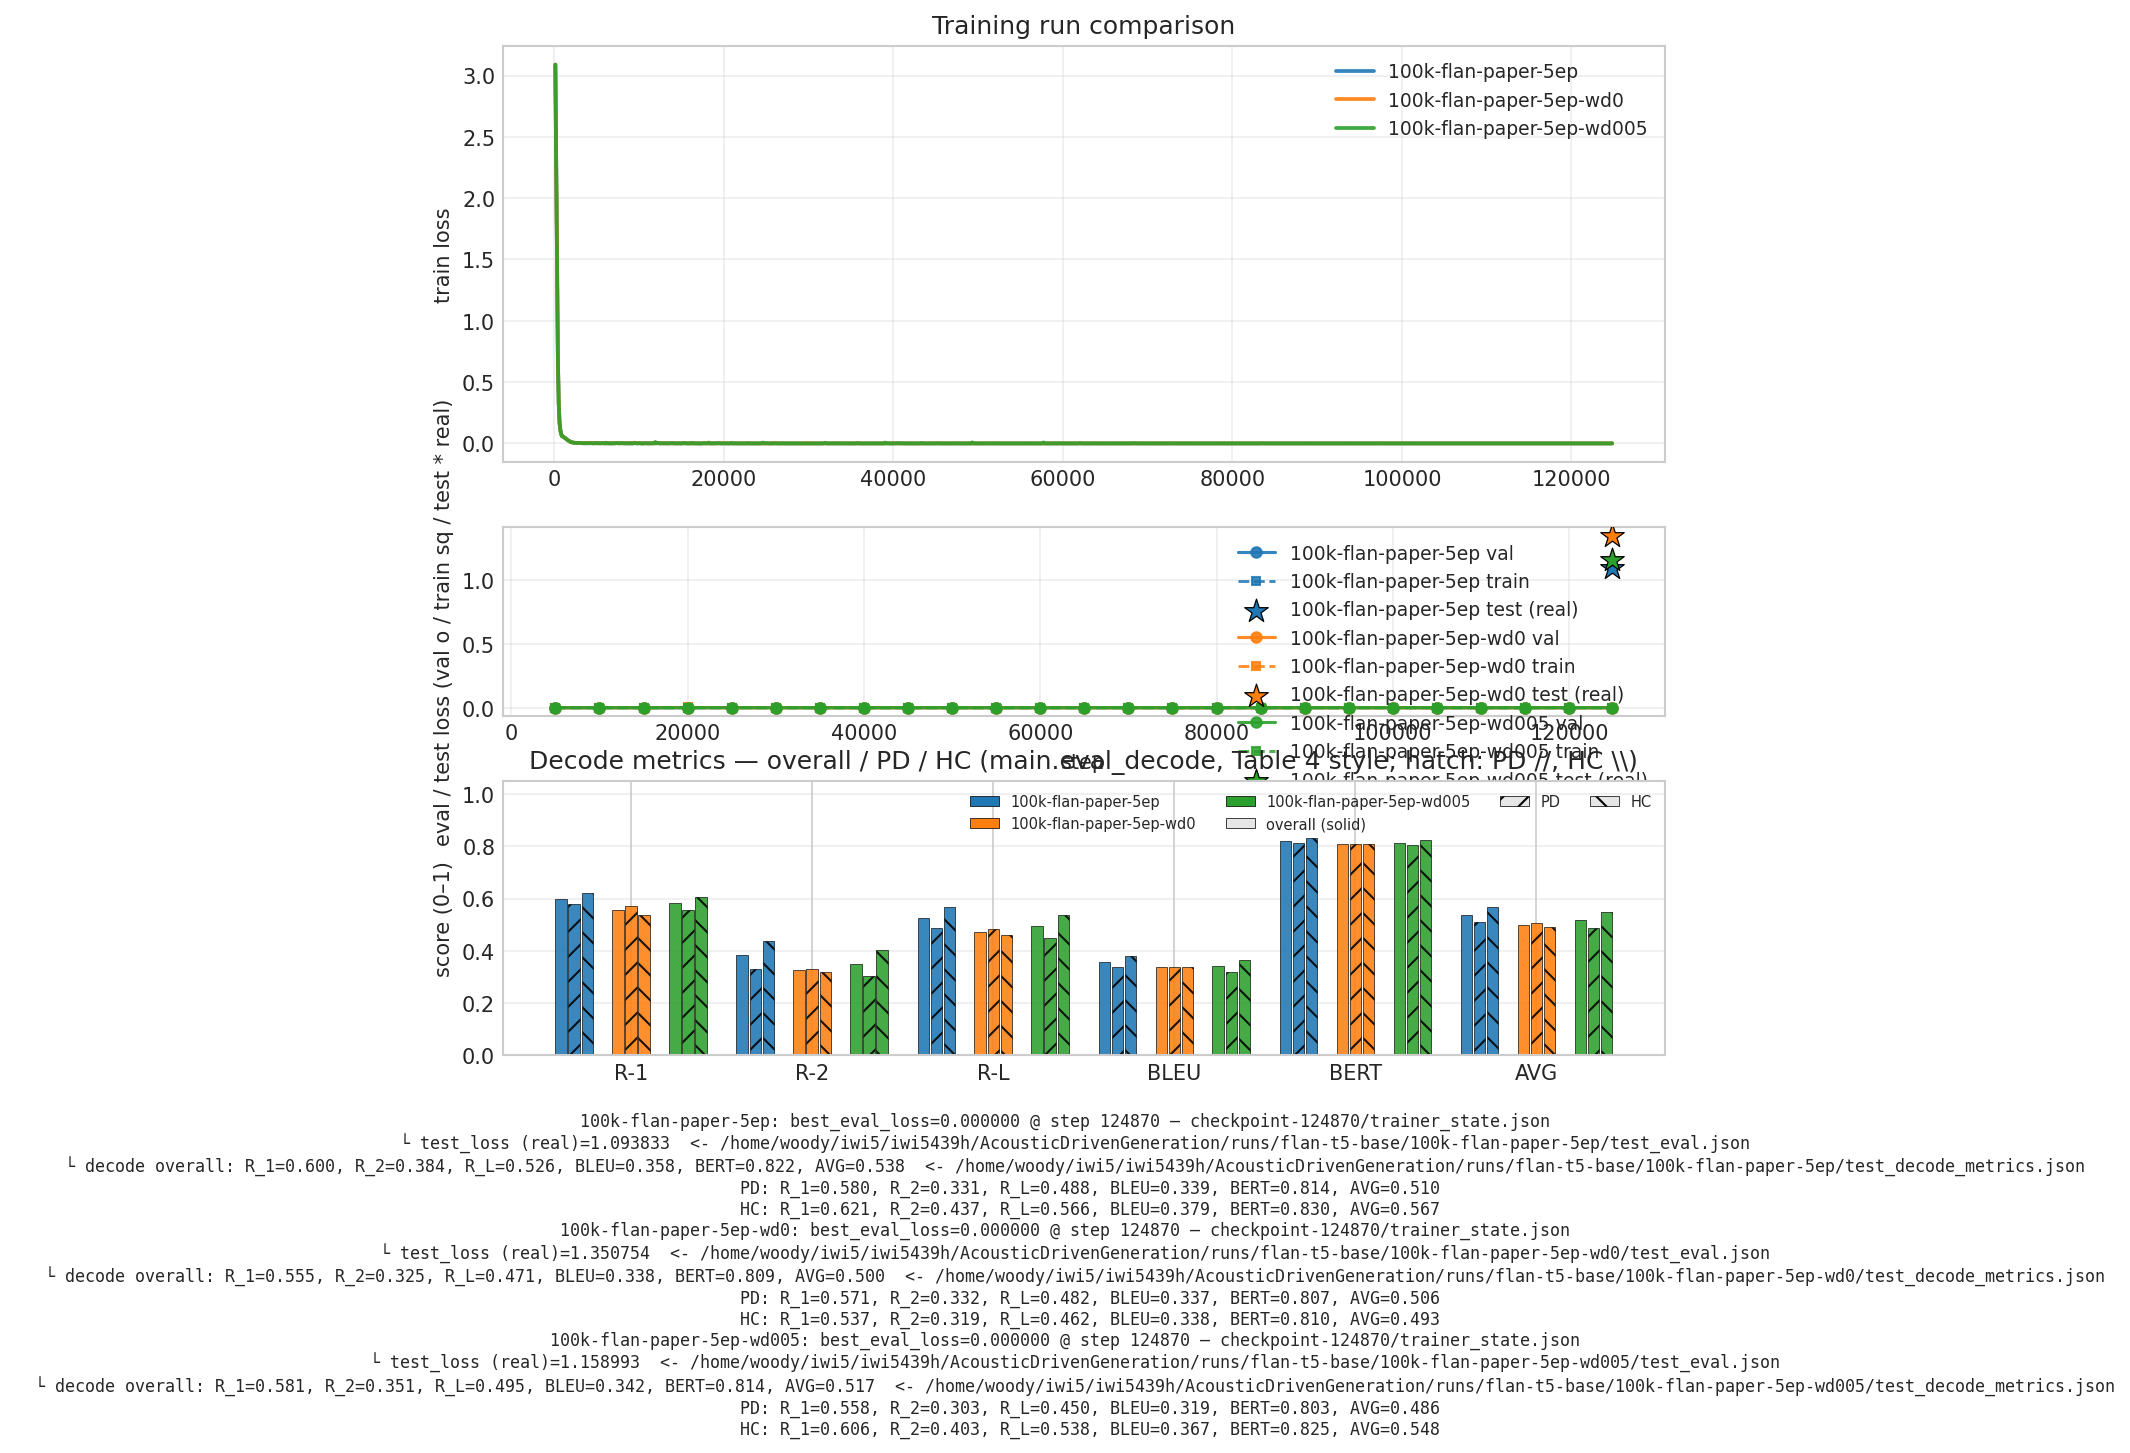
\includegraphics[width=\columnwidth]{wd_sweep.png}
\caption{Weight-decay sweep at the B11 recipe (five epochs, \bt{flan-paper}, $5\mathrm{e}{-}4$).
Decay $0.01$ is best; both $0.0$ and $0.05$ regress, with the loss concentrated on the HC group.}
\label{fig:wd}
\end{figure}

\paragraph{Weight decay.}
A dedicated sweep (Figure~\ref{fig:wd}) shows $0.01$ is optimal: turning decay off drops AVG to
0.500 and raising it to 0.05 gives 0.517, both below B11's 0.538. The weight-decay lever is
therefore exhausted and fixed at 0.01.

\paragraph{Phase 4 --- adaptation.}
LoRA improves modestly with rank (r8 0.538, r16 0.540, r32 0.542); rank 32 (B17) is the best and
the rank sweep is closed. Longer LoRA (five epochs) ties it, and a decoder-only \bt{freeze-encoder}
run does not beat full B11. A non-Flan T5-base baseline (N0) regresses strongly (0.439),
confirming that instruction tuning is required. Tripling parameters to Flan-T5-large (L5) merely
ties base (0.536) at $3\times$ the cost, spending its extra capacity on HC while slightly hurting
PD.

\paragraph{Phase 5 --- structured generation.}
Forcing a seven-slot skeleton in post-processing (B21) raised slot coverage to 1.0 but dropped AVG
to 0.492; structure-aware re-ranking (B22) gave 0.531; training directly on label-only targets
(B23) collapsed prose quality (0.315). Severity oversampling (B20) tied B17.

\paragraph{Phase 6 --- encoder input.}
Feeding the raw, unparsed \bt{Instructions} string (B24) regressed to 0.479, confirming that the
compact seven-score input is the better encoder representation.

\begin{table}[t]
\centering
\caption{Selected closed levers (honest decode AVG, word-BLEU ruler; B17 $=$ 0.542 as originally
logged). None improved on B17.}
\label{tab:levers}
\footnotesize
\setlength{\tabcolsep}{4pt}
\begin{tabularx}{\columnwidth}{@{}lYc@{}}
\toprule
Lever & Configuration & AVG \\
\midrule
Learning rate & $3\mathrm{e}{-}4$ / $5\mathrm{e}{-}4$ (base) & 0.395 / 0.522 \\
Epochs & 5 (B11) & 0.538 \\
LoRA rank & r8 / r16 / \textbf{r32} & 0.538 / 0.540 / \textbf{0.542} \\
Weight decay & 0.0 / \textbf{0.01} / 0.05 & 0.500 / \textbf{0.538} / 0.517 \\
Label smoothing & 0.02--0.10 & $\sim$0.176 \\
Model size & Flan-T5-large, 5 ep & 0.536 \\
Backbone & non-Flan T5-base & 0.439 \\
Oversampling & Moderate+ $2\times$ & 0.542 \\
Structured & post-proc / rerank / targets & 0.492 / 0.531 / 0.315 \\
Encoder input & raw \bt{Instructions} & 0.479 \\
\bottomrule
\end{tabularx}
\end{table}

\begin{figure}[t]
\centering
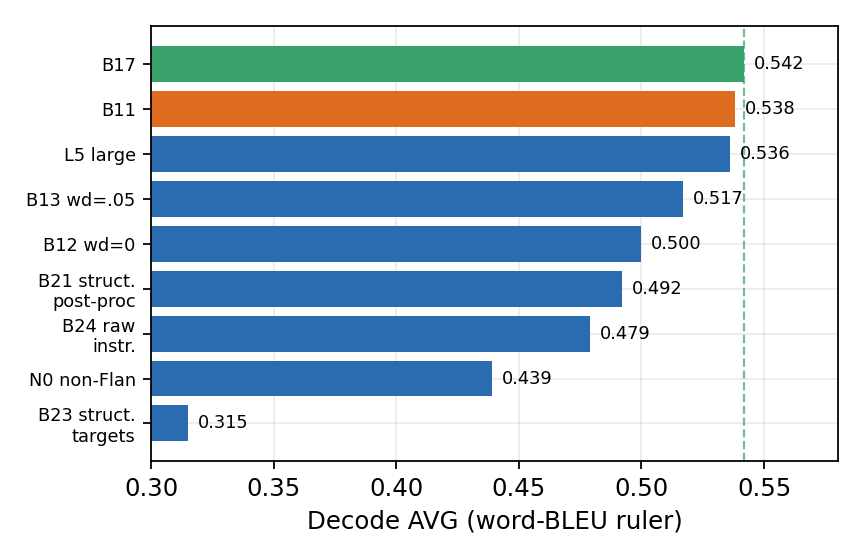
\includegraphics[width=\columnwidth]{fig_levers.png}
\caption{Honest decode AVG for representative configurations. The dashed line marks B17 (0.542,
as originally logged). Every alternative axis lands at or below B17.}
\label{fig:levers}
\end{figure}

\begin{figure}[t]
\centering
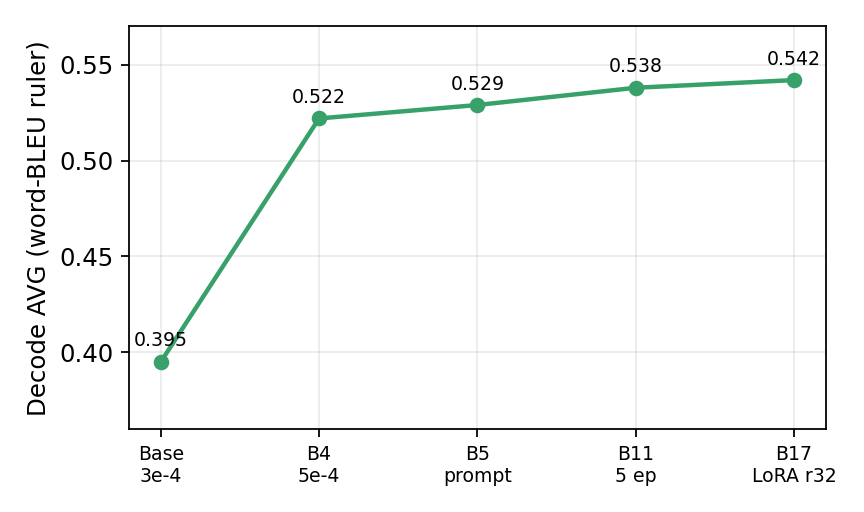
\includegraphics[width=\columnwidth]{fig_progression.png}
\caption{Decode AVG across the main configuration search on 100k data. The largest single gain is
the learning-rate change; prompt, epochs, and LoRA add smaller increments up to the plateau.}
\label{fig:progression}
\end{figure}

\begin{table}[t]
\centering
\caption{Condensed experiment log (honest decode AVG, as originally logged). ``$\Delta$'' is
relative to B17.}
\label{tab:full}
\small
\begin{tabular}{llcc}
\toprule
ID & Description & AVG & $\Delta$ \\
\midrule
Base & 100k, $3\mathrm{e}{-}4$ & 0.395 & $-0.147$ \\
B4 & 100k, $5\mathrm{e}{-}4$ & 0.522 & $-0.020$ \\
B5 & $+$ \bt{flan-paper} prompt & 0.529 & $-0.013$ \\
B6 & $+$ category hints & 0.509 & $-0.033$ \\
B7 & $+$ numeric labels & 0.460 & $-0.082$ \\
B11 & 5 epochs & 0.538 & $-0.004$ \\
B12 & weight decay 0.0 & 0.500 & $-0.042$ \\
B13 & weight decay 0.05 & 0.517 & $-0.025$ \\
B16 & LoRA r8 & 0.538 & $-0.004$ \\
\textbf{B17} & \textbf{LoRA r32} & \textbf{0.542} & \textbf{---} \\
B18 & LoRA r32, 5 ep & 0.542 & $0.000$ \\
B20 & $+$ oversampling & 0.542 & $0.000$ \\
B21 & structured post-proc & 0.492 & $-0.050$ \\
B23 & label-only targets & 0.315 & $-0.227$ \\
B24 & raw \bt{Instructions} & 0.479 & $-0.063$ \\
L5 & Flan-T5-large, 5 ep & 0.536 & $-0.006$ \\
N0 & non-Flan T5-base & 0.439 & $-0.103$ \\
S4 & Flan-T5-small (best) & 0.437 & $-0.105$ \\
\bottomrule
\end{tabular}
\end{table}

\subsection{PD versus HC}
Across both rulers, HC reports are generated more accurately than PD reports
(Figure~\ref{fig:pdhc}): under the parity ruler, HC AVG is 0.674 versus PD 0.623, and HC
character-BLEU 0.775 versus PD 0.744. This mirrors the reference paper's own observation that
models perform better on HC data, and is consistent under our honest metric as well. PD reports
describe more heterogeneous, severe impairment patterns, which are harder to reproduce verbatim.

\begin{figure}[t]
\centering
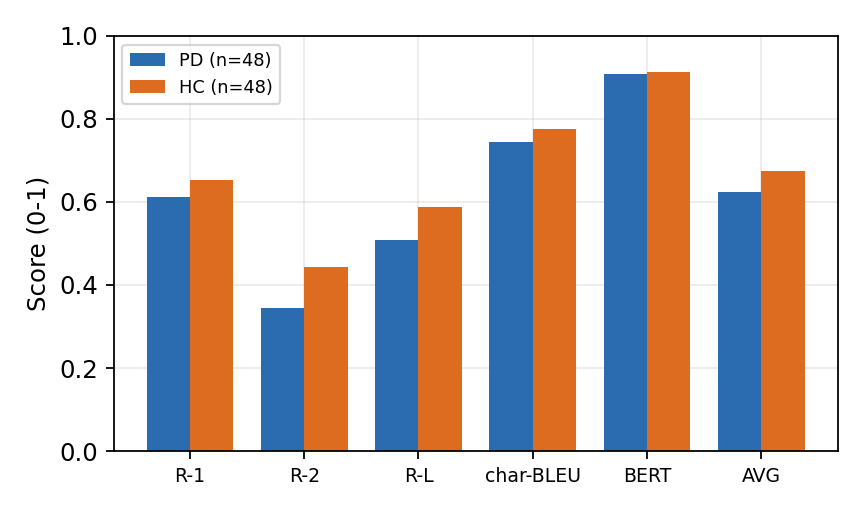
\includegraphics[width=\columnwidth]{fig_pd_hc.png}
\caption{PD versus HC under the author-parity ruler. HC reports are consistently easier across
every metric, matching the reference study's observation.}
\label{fig:pdhc}
\end{figure}

\subsection{Structure coverage}
Although generated reports read fluently and score well, strict parsing shows that only about 14\%
of generated texts contain all seven explicit \bt{Category (Severity)} slots, versus 100\% in the
references. Attempts to force this structure (post-processing, re-ranking, and training directly
on structured or label-only targets) improved slot coverage but did \emph{not} improve overall
decode quality---and structured targets sharply reduced it (AVG 0.315). The remaining gap to the
reference's 7B systems is therefore best understood as a problem of \emph{scale and structured
generation}, not of further small-model hyperparameter tuning.

\begin{figure}[t]
\centering
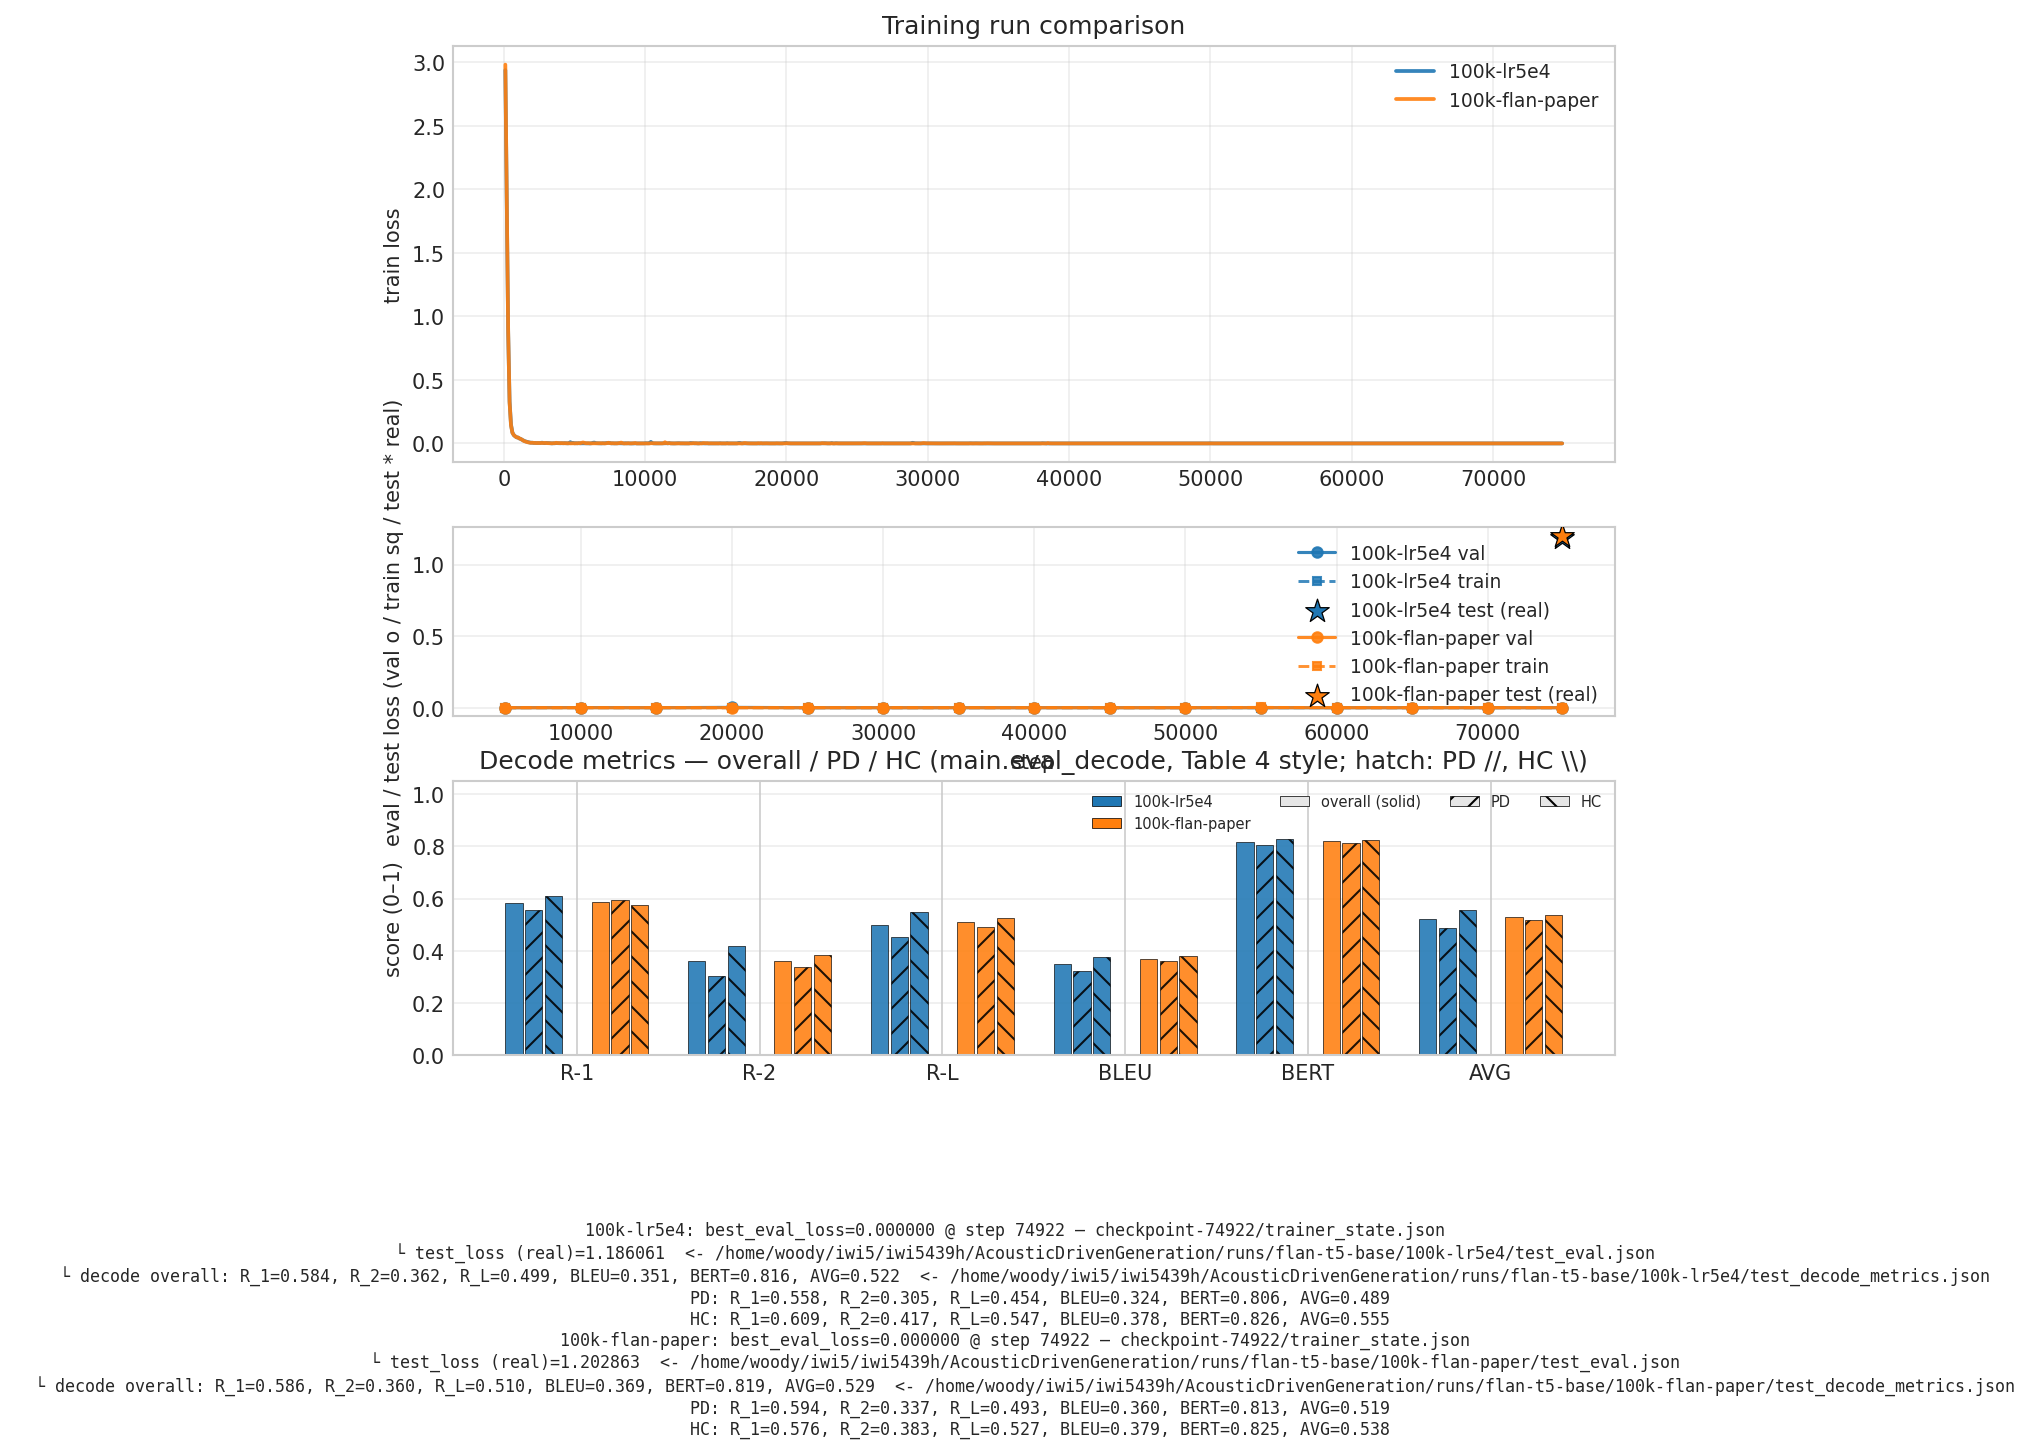
\includegraphics[width=\columnwidth]{training_curves.png}
\caption{Representative training/validation curves for base-scale runs, illustrating the
loss-versus-generation decoupling that motivates selecting checkpoints by decode AVG rather than
validation loss.}
\label{fig:curves}
\end{figure}

\subsection{Qualitative analysis}
The input and target share a fixed, human-readable structure, which is worth making concrete.
The encoder input is the task prefix followed by the seven biomarker values; the target is an
mFDA report in which each of the seven categories appears as a \bt{Category (Severity):} clause
followed by a short clinical description. A representative pairing (format-accurate; values
illustrative) is:

\vspace{0.3em}
\noindent\fbox{\begin{minipage}{0.93\columnwidth}\footnotesize
\textbf{Input (encoder):}\\
\texttt{Generate a report for: Breathing: 78 Lips: 1.75 Palate: 0.94 Larynx: 5.42 Monotonicity: 62.3 Tongue: 0.19 Intelligibility: 0.72}
\vspace{0.3em}\\
\textbf{Target (reference report):}\\
\textit{Breathing (Severe): control over respiration is grossly distorted. Lips (Mild):
inconsistent lip closure, but overall good control. Palate (Moderate): some impairment is
noticeable, but speech production happens with a reasonable approximation. Larynx (Severe):
unable to maintain proper intonation and loudness. Monotonicity (Mild): minimal difficulty
changing tone \dots}
\end{minipage}}
\vspace{0.4em}

Qualitatively, B17 generations are fluent, clinically plausible, and reproduce the
\bt{Category (Severity)} pattern for the most salient categories; this is why embedding-based and
$n$-gram overlap scores are relatively high. However, they frequently omit or merge some of the
seven explicit slots---only about 14\% contain all seven---so while the coarse severity picture is
usually right, the model does not reliably emit the full structured skeleton. This mismatch
between fluent-but-incomplete generation and the fully-slotted references is the qualitative
counterpart to the quantitative structure-coverage result, and it is what the (unsuccessful)
structured-generation experiments in Phase 5 attempted to address.

\section{Discussion and Limitations}
The headline outcome is that a careful, standardised evaluation changes the story completely.
Measured with a common word-level BLEU and an English BERTScore, B17 attains AVG 0.559; measured
with the reference paper's own character-level BLEU, the same model attains AVG 0.649---close to
seven-billion-parameter systems. The lesson generalises beyond this project: \emph{when comparing
generation systems, the metric implementation must be reproduced, not merely named.} A single
undocumented choice (character versus word BLEU, or the BERTScore backbone language) can move a
reported score by tens of points and completely reframe a model's apparent competitiveness. For
any comparison a student or reviewer presents, the safe practice is to run the reference
evaluation code---or a faithful reimplementation of it---on the new model, which is exactly what
our author-parity harness provides.

A secondary but practically important finding is the decoupling of teacher-forcing loss from
generation quality. On several occasions a checkpoint with the lowest synthetic validation loss
did not produce the best decoded reports---in one case a step with near-zero validation loss was
edged on decode AVG by a later checkpoint---and low test loss did not guarantee high BLEU/ROUGE.
This is a well-known but frequently ignored pitfall: cross-entropy rewards matching the reference
token-by-token under teacher forcing, whereas beam or sampled generation is evaluated on whole
sequences against $n$-gram and embedding metrics. Throughout the study we therefore treat decode
AVG as the sole selection criterion and use validation loss only as a coarse training-health
signal. Any reproduction of this work should do the same; selecting by loss would have chosen
different, worse checkpoints at several points.

Several limitations qualify these results. First, the synthetic training corpus is highly
templated and repetitive (duplicate rate 0.95), so the model may partly memorise phrasing rather
than learn a robust biomarker-to-severity mapping; the varied real test reports expose this. This
distribution mismatch, not model capacity alone, likely bounds achievable overlap scores. Second,
the author-parity decode uses sampling, so its numbers vary slightly between runs; we report a
single seeded run. Third, our comparison to the paper's 0.789/0.836 is to its \emph{best} (7B)
systems; the paper's exact Flan-T5 cell was not available to us, though our parity numbers
strongly suggest B17 matches or exceeds a comparable Flan-T5. Fourth, BLEU, ROUGE, and even
BERTScore reward surface and embedding similarity, not clinical correctness; a report can score
well while mislabelling a severity, so these metrics are proxies for report quality, not clinical
validation. Finally, the test set is small (96 reports), so PD/HC differences of a few points
should be interpreted cautiously.

\section{Ethical and Clinical Considerations}
Because the ultimate application is clinical, several considerations bound how such a system
should be used. First, the evaluation metrics reported here---BLEU, ROUGE, BERTScore---measure
textual similarity, not diagnostic correctness. A generated report can be fluent and score highly
while assigning the wrong severity to a category; consequently the model should be positioned as a
\emph{decision-support and drafting aid} that a clinician reviews and corrects, never as an
autonomous diagnostic instrument. Second, the training data are synthetic by design, simulated
from the statistical distribution of a small real cohort (100 subjects) from a single corpus
(PC-GITA, Colombian-Spanish speakers). Models trained this way may not transfer to other
languages, recording conditions, dysarthria aetiologies, or demographic groups, and could encode
the biases of the simulation and of the three expert raters whose median scores define the
targets. Third, clinical reports are sensitive data; the pipeline keeps real reports isolated to
the test split and version-controls only compact metric artifacts, never the reports or model
weights, but any deployment would require appropriate data-governance safeguards. Finally, the
tendency of language models to produce confident, plausible text means an incomplete or incorrect
report may read as authoritative; surfacing the seven input biomarkers alongside every generated
report---so a clinician can trace each statement back to its acoustic evidence---is an important
mitigation and a further argument for the structured, slot-based generation proposed as future
work.

\subsection*{Threats to validity}
The main internal threat is the train/test distribution mismatch (templated synthetic training
versus varied real reports), which caps overlap metrics regardless of model quality. The main
external threat is single-corpus, single-language data. A construct-validity threat is that all
three metrics are proxies for report quality; a small expert human evaluation of a sample of
generated reports would strengthen the conclusions and is recommended before any clinical piloting.

\section{Conclusion and Future Work}
This project delivered a reproducible pipeline and a best Flan-T5 model (B17: Flan-T5-base with
rank-32 LoRA) for generating mFDA-style clinical speech reports from seven acoustic biomarkers,
together with a systematic map of what does and does not help this task. Its most important
result is methodological: the apparent gap between our compact model and the reference paper was
\emph{mostly a measurement artifact}. Under the paper's own metric, a 248M model is competitive
with systems roughly 28$\times$ larger; the gap shrinks from ``far behind'' to a few points once
BLEU is computed the same way and BERTScore uses the correct language. We additionally corrected a
BERTScore language misconfiguration that had systematically undervalued semantic scores, and we
documented the closed levers so future work does not re-explore them.

For the Flan-T5 track, B17 is final: every tuning axis we examined is saturated. Three directions
remain for future work. (i) \emph{Structured generation}: constrained or template-guided decoding
that guarantees all seven slots, potentially improving both interpretability and clinical
usefulness without harming fluency. (ii) \emph{Better training data}: reducing the synthetic
duplicate rate and increasing linguistic diversity to close the train/test distribution gap.
(iii) \emph{Scale}: moving to a decoder-only 7B model (e.g.\ LLaMA or Mistral) with LoRA---the
same family that produced the reference headline---which is the only route likely to surpass
0.789/0.836. Across all three, the standardised, reproducible evaluation established here should
be the basis for comparison, so that future gains reflect the model and not the ruler.

\section*{Reproducibility}
All results are reproducible from the project repository. The honest and author-parity metrics
for B17 are regenerated with \bt{main.eval\_decode} and \bt{main.eval\_author\_parity} on the
merged \bt{final\_model}; both write JSON artifacts with full per-example diagnostics. The ETL,
preparation, training, and evaluation stages are documented in the accompanying \bt{docs/} and run
deterministically under fixed seeds. The BERTScore English backbone (RoBERTa-large) must be cached
before offline evaluation on compute nodes; the author-parity script degrades to BLEU and ROUGE
with an explicit status flag if it is unavailable.

\appendix

\section{Pipeline command reference}
\label{app:cmd}
The full pipeline is driven by four commands, each a thin, documented entry point. Paths are
repo-relative.

\vspace{0.3em}
\noindent\textbf{1. ETL} --- raw CSVs to canonical Parquet/JSONL:
{\footnotesize\begin{flushleft}\ttfamily
python etl/run\_etl.py --train-size 100k
\end{flushleft}}

\noindent\textbf{2. Prepare} --- canonical splits to a tokenised \bt{DatasetDict}:
{\footnotesize\begin{flushleft}\ttfamily
python -m main.prepare \\
\hspace*{1em}--output-dir data/processed/flan-t5-base/100k-flan-paper \\
\hspace*{1em}--train-size 100k --prompt-style flan-paper \\
\hspace*{1em}--tokenize --tokenizer-model google/flan-t5-base
\end{flushleft}}

\noindent\textbf{3. Train} --- \bt{Seq2SeqTrainer} with optional LoRA:
{\footnotesize\begin{flushleft}\ttfamily
python -m main.train \\
\hspace*{1em}--tokenized-dir .../100k-flan-paper/tokenized \\
\hspace*{1em}--output-dir runs/flan-t5-base/100k-flan-paper-5ep \\
\hspace*{1em}--model-name google/flan-t5-base \\
\hspace*{1em}--num-train-epochs 5 --learning-rate 5e-4 \\
\hspace*{1em}--weight-decay 0.01 --require-gpu
\end{flushleft}}

\noindent\textbf{4. Evaluate} --- both rulers on the merged \bt{final\_model}:
{\footnotesize\begin{flushleft}\ttfamily
python -m main.eval\_decode ... --require-gpu \\
python -m main.eval\_author\_parity ... --require-gpu
\end{flushleft}}

\noindent The LoRA (B17) stage sets \bt{--lora-rank 32} and \bt{--model-name} to the B11
\bt{final\_model}; adapters are merged on save so evaluation is unchanged.

\section{Detailed split audit}
\label{app:audit}
Table~\ref{tab:app-audit} gives the per-split audit underlying Section~\ref{sec:results}. All
seven mFDA categories are present in 100\% of reports across every split; the distinguishing
factor is the target duplicate rate, which is very high for the templated synthetic corpus and
much lower for the varied real reports.

\begin{table}[h]
\centering
\caption{Per-split structure and length audit (all seven categories present at rate 1.0).}
\label{tab:app-audit}
\small
\begin{tabular}{lccc}
\toprule
Property & Train & Val & Test \\
\midrule
$n$ & 99{,}893 & 10{,}000 & 96 \\
Real data & no & no & yes \\
Category coverage & 1.00 & 1.00 & 1.00 \\
All-7-slots rate & 1.00 & 1.00 & 1.00 \\
Median length (chars) & 494 & 494 & 438 \\
Mean length (chars) & 501.5 & 501.9 & 449.1 \\
Duplicate target rate & 0.949 & 0.845 & 0.500 \\
\bottomrule
\end{tabular}
\end{table}

\noindent Within the test split, PD reports are longer (median 478 characters) than HC reports
(median 404), consistent with PD reports describing more (and more severe) abnormal categories.

\section{Prompt styles}
\label{app:prompts}
Five encoder task-prefix styles were implemented and compared (Section~\ref{sec:results},
Phase 2):
\begin{itemize}[leftmargin=1.2em,itemsep=0.12em,topsep=0.2em]
  \item \textbf{default} --- an explicit mFDA biomarker instruction.
  \item \textbf{flan-paper} --- the reference prefix ``Generate a report for:'' over the compact
        seven-score input; the best style and the B5/B11/B17 default.
  \item \textbf{flan-paper-categories} --- the paper prefix plus explicit seven-category hints
        (B6); regressed.
  \item \textbf{flan-paper-numeric-labels} --- deterministic \bt{Category=value} formatting (B7);
        regressed most, concentrated on HC.
  \item \textbf{flan-paper-report-template} --- a seven-slot \bt{Category (Severity):} output
        template (B19); no improvement.
\end{itemize}

\section{Experiment provenance and compute}
\label{app:compute}
Every run carries an identifier (B$n$ for Flan-T5-base; S, L, N prefixes for small, large, and
non-Flan) that is kept in sync across three documents---the recipe, the results log, and the
roadmap---and after which the corresponding batch scripts are named. This convention makes each
number in the results traceable to an exact configuration and artifact. Training and evaluation
run on the NHR@FAU TinyGPU cluster: A100 (40\,GB) nodes for base and large models, with V100 and
RTX~3080 partitions as fallbacks; FP16 is avoided on V100 for numerical stability. Because compute
nodes are offline, Hugging Face model weights---including the RoBERTa-large BERTScore
backbone---are pre-cached on the login node before batch evaluation. Only compact metric JSON
artifacts are version-controlled; multi-gigabyte checkpoints remain on the cluster. The
model-selection rule throughout is to rank configurations by decode AVG from \bt{eval\_decode},
never by teacher-forcing validation loss, which repeatedly diverged from generation quality.

\begin{thebibliography}{99}
\small
\bibitem{ariasvergara2025} T.\ Arias-Vergara et al., ``Acoustic-Driven Generation of Pathological
Speech Reports Using Large Language Models,'' preprint, DOI 10.21203/rs.3.rs-7326708/v1, 2025.
\bibitem{raffel2020} C.\ Raffel et al., ``Exploring the Limits of Transfer Learning with a Unified
Text-to-Text Transformer,'' \emph{JMLR}, 21(140):1--67, 2020.
\bibitem{chung2022} H.\ W.\ Chung et al., ``Scaling Instruction-Finetuned Language Models,''
arXiv:2210.11416, 2022.
\bibitem{hu2021} E.\ J.\ Hu et al., ``LoRA: Low-Rank Adaptation of Large Language Models,''
\emph{ICLR}, 2022.
\bibitem{papineni2002} K.\ Papineni, S.\ Roukos, T.\ Ward, and W.-J.\ Zhu, ``BLEU: A Method for
Automatic Evaluation of Machine Translation,'' \emph{ACL}, 2002.
\bibitem{lin2004} C.-Y.\ Lin, ``ROUGE: A Package for Automatic Evaluation of Summaries,'' \emph{ACL
Text Summarization Workshop}, 2004.
\bibitem{zhang2020} T.\ Zhang, V.\ Kishore, F.\ Wu, K.\ Q.\ Weinberger, and Y.\ Artzi,
``BERTScore: Evaluating Text Generation with BERT,'' \emph{ICLR}, 2020.
\bibitem{post2018} M.\ Post, ``A Call for Clarity in Reporting BLEU Scores,'' \emph{WMT}, 2018.
\bibitem{liu2019} Y.\ Liu et al., ``RoBERTa: A Robustly Optimized BERT Pretraining Approach,''
arXiv:1907.11692, 2019.
\bibitem{orozco2014} J.\ R.\ Orozco-Arroyave et al., ``New Spanish Speech Corpus Database for the
Analysis of People Suffering from Parkinson's Disease (PC-GITA),'' \emph{LREC}, 2014.
\bibitem{wolf2020} T.\ Wolf et al., ``Transformers: State-of-the-Art Natural Language
Processing,'' \emph{EMNLP: System Demonstrations}, 2020.
\bibitem{touvron2023} H.\ Touvron et al., ``LLaMA: Open and Efficient Foundation Language
Models,'' arXiv:2302.13971, 2023.
\bibitem{jiang2023} A.\ Q.\ Jiang et al., ``Mistral 7B,'' arXiv:2310.06825, 2023.
\bibitem{radford2019} A.\ Radford et al., ``Language Models are Unsupervised Multitask Learners''
(GPT-2), OpenAI Technical Report, 2019.
\end{thebibliography}

\end{document}
